%================================================================
\section{Comics Theory}

The basis of McCloud's theory about making sense of panel sequences across
the gutters, later validated experimentally, is that
readers of comics optimize their
consumption of relevant information~\cite{pirolli2007information}, and work
to construct inferences~\cite{magliano2016filling} about story content in
these liminal spaces of discourse.
% (in between sentences in text, panels in
% comics, scenes in film). 
Inferences for story content are constructed when
they are needed for comprehension and enabled by what has
been narrated thus far~\cite{myers1987degree}. The dynamic
between story authors and audiences parallels the dynamics of people
engaged in cooperative conversation as outlined by the philosopher of
language Grice~\cite{grice1975logic}: the storyteller, as the active contributor
to the ongoing communicative context, is expected to make her contributions
to the discourse based on what is relevant to her narrative intent. 
McCloud's introduced six {\em
panel transition types} for comics~\cite{mcCloud1993understanding}, 
enumerate the different roles that the reader may infer from a
well-written comic. These transition types are {\em moment-to-moment}, {\em
action-to-action}, {\em subject-to-subject}, {\em aspect-to-aspect}, {\em
scene-to-scene}, and non sequitur. While it is tempting to think we could
simply operationalize these transitions in a generator, as
Cohn~\cite{cohn2013visual} (Chapter 4) points out, so much of their meaning
relies on contextual, real-world-situated understanding that it lends
little help to computational authoring.

% However, other scholars have identified that comics are structurally similar to written
% text~\cite{saraceni2016relatedness}: they are both made up of individual
% elements (sentences in text, panels in comics), delimited by special-purpose
% symbols (full stops in text, panel borders in comics), which can be easily
% identified, and which can contain a variable amount of information. However,
% unlike text, comics also express information via visual elements and their spatial
% relationships to one another, which we might model in terms of their
% relative size, rotation, horizontal and vertical juxtaposition, and
% distance. While in general comics offer two dimensions of authorship
% affordances (textual and visual language), in this work we are concerned
% only with the pictorial dimension.
%
\begin{figure}
	\centering
	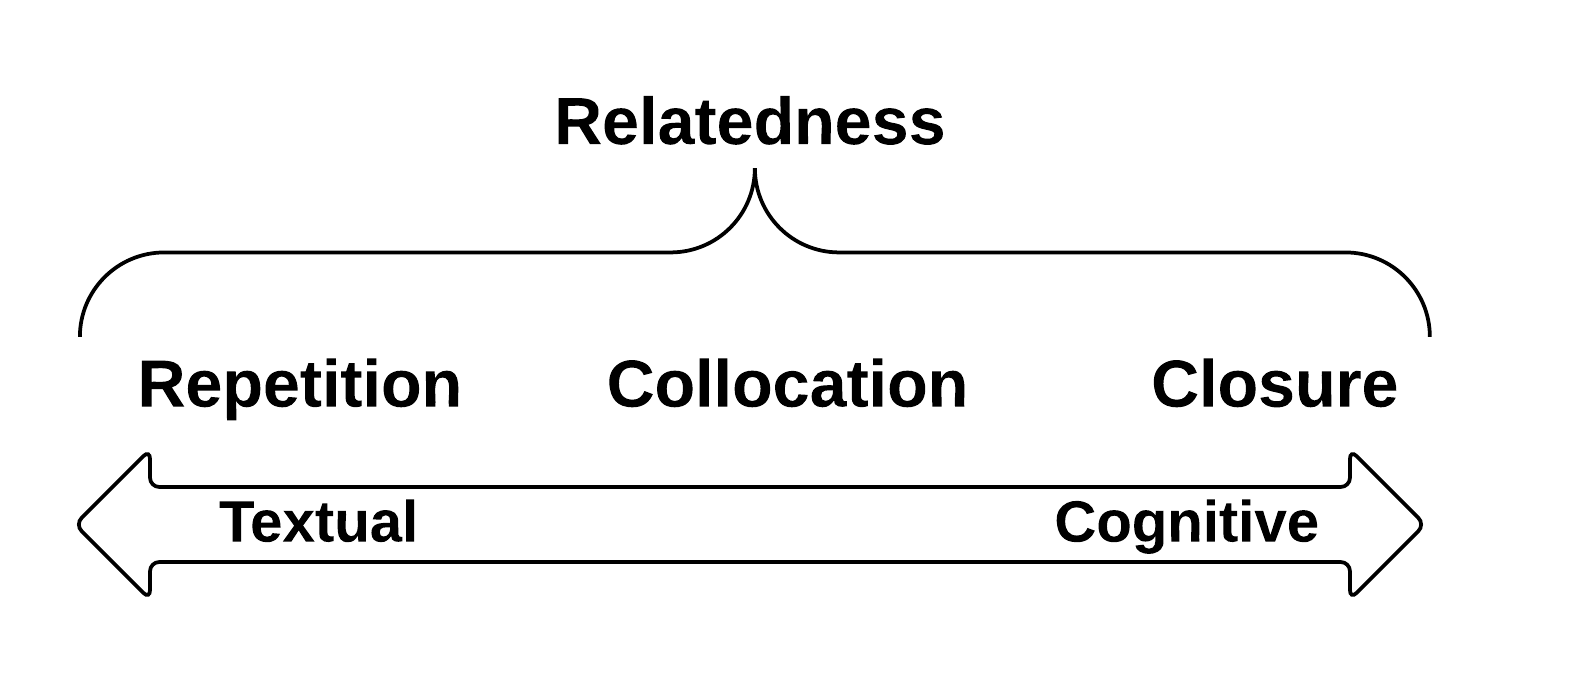
\includegraphics[width=0.5\columnwidth]{relatedness.png}
	\caption{
		The spectrum of \emph{relatedness} as discussed by
                Saraceni~\cite{saraceni2016relatedness}. Relatedness indicates how 
		comic panels are connected or associated in the minds of 
		readers, spanning from textual factors to cognitive factors. 
		Along that spectrum, there are three  distinguished 
		categories of relatedness: \emph{repetition}, 
		\emph{collocation}, and \emph{closure}, which have
		demonstrably different effects on the construction of
		narrative mental models.
		}
	\label{figure:relatedness}
\end{figure}
%

However, Saraceni~\cite{saraceni2016relatedness} supports
McCloud's hunch that readers create meaning from comics from perceived
relationships between panels.  Saraceni describes three notions of
\emph{relatedness} between comic elements, which are the building blocks
from which readers may construct meaning inferences.  
Relatedness creates  a comic's \emph{cohesion} -- the lexico-grammatical
features that tie panels together -- and \emph{coherence} -- the audience's
perception of how individual panels contribute to her mental model of the
unfolding events. Relatedness emerges from a spectrum of
\emph{textual}\footnote{\emph{Textual} here does not mean the use of actual
text, but rather is a shorthand for \emph{surface
code}~\cite{zwaan1998situation}.} factors to \emph{cognitive} factors,
illustrated in \fref{figure:relatedness}.
%
% Saraceni distinguishes three categories of relatedness.  
Closer to the textual end of the spectrum is the \emph{repetition} of
visual elements across panels. Beyond repetition is \emph{collocation},
which refers to an audience's expectation that related visual elements will
appear given the ones that have been perceived. Closer to the cognitive end
of the spectrum is the \emph{closure} over comic elements, which refers to
the way our minds complete narrative material given to us. Closure is
terminologically borrowed from the field of visual cognition, but is
intended as the mental process of inference that occurs as part of an
audience's \emph{search for meaning}~\cite{gerrig1994readers}.

%
% \begin{figure}[t]
%   \centering
% 	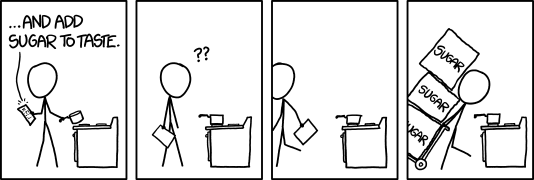
\includegraphics[width=9cm]{xkcd-to_taste.png}
% 	\caption{
% 		Strip \#1639 of {\em XKCD}, {\small\copyright} Randall Munroe. This comic
% 		depends on three aspects of relatedness as described by 
%                 Saraceni~\cite{saraceni2016relatedness}, and as illustrated in 
% 		\fref{figure:relatedness}.
% 	}
% \label{fig:xkcd}
% \end{figure}
The comic in Figure~\ref{fig:calvin} depends on these three 
aspects of relatedness: first, repetition of the sled, snowman, and other
figures maintains cohesion across panels. Second, the humor of the sled
carrying off the snowman depends on our (non-grammatical) domain knowledge
that the snowman is not a living character in the same sense as the other
figures. Finally, the comic depends on closure for the audience to ``fill
in the gaps'' to infer what must have happened during the ``WUMP!'' panel:
the sled maintained momentum to carry off the snowman, and the riders of
the sled landed on top of the girl.

%================================================================
\section{Related Work}

In terms of visual storytelling,
Heider and Simmel~\cite{heider1944experimental} formulated an experiment
based on abstract shapes in animation and evaluated whether audiences
perceived consistent stories. Their work also depends on cognitive closure
to achieve a narrative goal; however, the animations themselves were
hand-authored rather than generated.
Pioneering work on visual discourse by Jhala and
Young~\cite{jhala2005discourse} addresses visual storytelling in terms of camera
control for cinema-style storytelling. We consider the representation
and generation strategies emerging from this work~\cite{jhala2010cinematic}
as strong candidates for future work in terms of scene specification;
however, we look to comics as a simpler, more discretize domain that does
not depend on a deeply simulated underlying narrative.

P\'erez y P\'erez et al.~\cite{perezyperez2012illustrating} developed a 
visual illustrator to the MEXICA system~\cite{perez2001mexica}, and verified
%
the degree to which their 3-panel comic generator 
elicited in readers the same sense of story as a textual realization of 
the same MEXICA-generated plot. 
%
While this system also follows the pipeline model of narrative generation,
we see their work as complementary: they developed an experiment
methodology through which it is possible to empirically assess if their
palette of designed visual elements denote story concepts as intended.
Future work in comic generation will have to address this point going
forward, and P\'erez y P\'erez et al. provide a step toward understanding
the gap between story concepts and the pictorial symbols meant to encode
them. 

% (XXX interacive comics)

%A potential improvement to their system that the authors 
%identify as most important was: ``to provide the Visual Narrator with mechanisms
%that allow more freedom during the composition 
%process''~\cite{perezyperez2012illustrating}. Our work here aims to provide just 
%that.



